\section{Theorie}
\label{sec:Theorie}

\subsection{Energieverteilung und Sättigungsstrom}

In einem Leiter können sich Elektronen nahezu frei bewegen. Um jedoch den Leiter verlassen zu können, müssen sie wie in dem in Abbildung \ref{fig:pot} dargestellten Potentialtopf die Potentialdifferenz $\phi$ überwinden, also eine Austrittsarbeit von $W_.A=\mathrm{e}_.0\phi$, mit der Elementarladung des Elektrons $\mathrm{e}_.0$, leisten. \newline
Die Energieverteilung ist mit der Fermischen Grenzenergie $\zeta$, der Temperatur $T$ und der Boltzmann-Konstante $k_.B$ gegeben durch die Fermi-Diracsche-Verteilungsfunktion
\[
f(E)= \frac{1}{\exp{\left(\frac{E-\zeta}{k_.BT}\right)}-1}\text{,}
\]
deren Verlauf für verschiedenen Temperaturen in Abbildung \ref{fig:fermi} dargestellt ist.
Die Elektronen müssen also mindestens die Energie $E_.0=\zeta + \mathrm{e}_.0\phi\gg k_.BT$ besitzen um das Material zu verlassen, weshalb die Verteilung zu 
\begin{equation}
f(E)\approx\exp{\left(\frac{-\mathrm{e}_.0\phi}{k_.BT}\right)}\label{eq:FDV}
\end{equation}
genähert werden kann. Da die Elektronen den Leiter nur verlassen können, wenn sie mindestens $E_.0$ als kinetische Energie in Normalenrichtung zur Leiteroberfläche $A$ aufweisen, muss für die Sättigungsstromdichte $j_.S$ über alle Elektronen integriert werden, die diese Energie besitzen. Damit ergibt sich für $j_.S$ die Richardson-Gleichung
\[
j_.S(T)=4\pi\frac{\mathrm{e}_.0m_.0k^2_.B}{h^3}T^2\exp{\left(\frac{-\mathrm{e}_.0\phi}{k_.BT}\right)}
\]
und mit $I=j\cdot A$ für den Sättigungsstrom 
\begin{equation}
I_.S(T) = 4\pi A\frac{\mathrm{e}_.0m_.0k^2_.B}{h^3}T^2\exp{\left(\frac{-\mathrm{e}_.0\phi}{k_.BT}\right)}\text{.}
\end{equation}
Das Plancksche Wirkungsquantum $h$ kommt dabei daher, das jeder Energiezustand im Phasenraum ein Volumen von $h^3$ einnimmt.

\begin{figure}
\centering
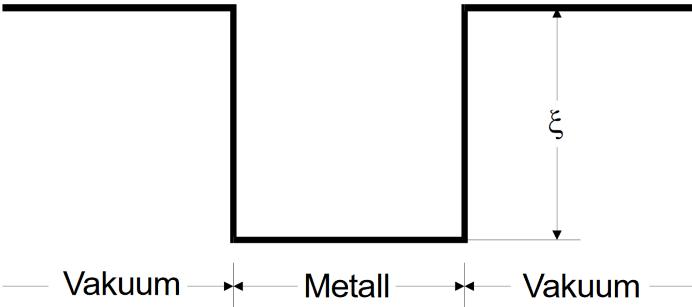
\includegraphics[width=\linewidth-70pt,height=\textheight-70pt,keepaspectratio]{content/images/Pot.jpg}
\caption{Modell eines Potentialtopfs mit Whandhöhe $\xi = \phi$ zur Beschreibung der Potentialverhältnisse in einem Leiter\cite{V504}}
\label{fig:pot}
\end{figure}

\begin{figure}
\centering
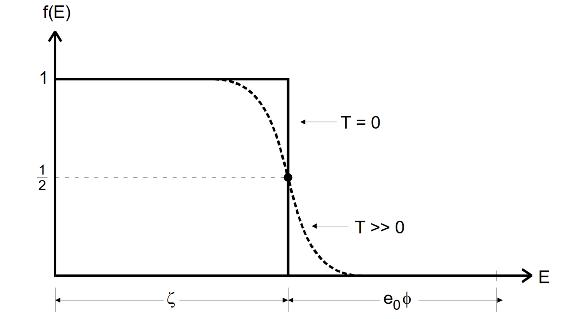
\includegraphics[width=\linewidth-70pt,height=\textheight-70pt,keepaspectratio]{content/images/fermi.jpg}
\caption{Verlauf der Fermi-Dirac-Verteilung am absoluten Nullpunkt und für wesentlich größere Temperaturen\cite{V504}\label{fig:fermi}}
\end{figure}

\subsection{Die Hochvakuum-Diode}
\subsubsection{Aufbau}
\noindent Um Wechselwirkungen mit Luftmolekülen zu vermeiden, muss der Sättigungsstrom im Vakuum gemessen werden. Außerdem müssen die freiwerdenden Elektronen mit Hilfe eines elektrischen Feldes abgesaugt werden.
Bei einer Hochvakuumdiode wird dazu in einem evakuierten Glasbehälter zwischen dem über Heizspannung als Kathode betriebenen Glühdraht und einer Anode eine Spannung angelegt, wie in Abbildung \ref{fig:HVD}.

\begin{figure}
\centering
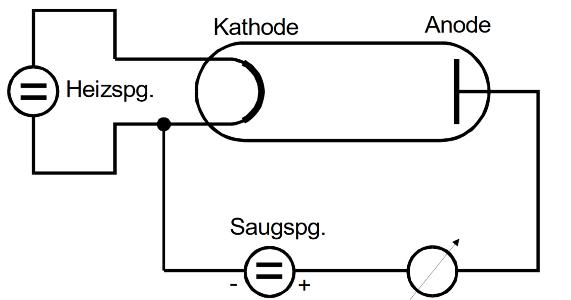
\includegraphics[width=\linewidth-70pt,height=\textheight-70pt,keepaspectratio]{content/images/HVD.jpg}
\caption{Schematischer Aufbau einer Hochvakuum-Diode\cite{V504}
\label{fig:HVD}}
\end{figure}
\subsubsection{Langmuir-Schottky-Gleichung und Anlaufstrom}
Beim Durchlaufen des Feldes zwischen Kathode und Anode werden die Elektronen beschleunigt und haben somit keine konstante Geschwindigkeit $v$.
Da aber die Stromdichte $j$ an jedem Punkt gleich ist, muss wegen $j=v\rho$
die Raumladungsdichte $\rho$ eine Funktion des Orts sein und in der Nähe der Anode geringer werden. Die Ladungsanhäufung in der Nähe der Kathode führt zu einer Schwächung des E-Felds, sodass für geringe Saugspannungen $V$ Langmuir-Schottky-Raumladungsgleichung gilt:
\begin{equation*}
j = \frac{4}{9}\epsilon_.0\sqrt{2\frac{e_.0V^3}{m_.0a^2}}
\end{equation*}
und somit
\begin{equation}
I = \frac{4}{9}A\epsilon_.0\sqrt{2\frac{e_.0V^3}{m_.0a^2}}<I_.S\text{.}
\label{eq:langmuir}
\end{equation}
Dabei beschreibt $a$ den Abstand zur Kathode.
Außerdem verfügen einige Elektronen bei der Freisetzung aus der Kathode über genügend kinetische Energie um sogar gegen ein geringes Gegenfeld zur Anode zu wandern und so einen Anlaufstrom zu erzeugen.
Je höher das Gegenfeld ist, desto geringer ist auch der Anlaufstrom:
\begin{equation}
I(V)=j_.0A\exp{\left(-\frac{e_.0\phi_.A+e_.0V}{k_.B	T}\right)}
\label{eq:Anlauf}
\end{equation}
$e_.0\cdot\phi_.A$ ist dabei die Austrittsarbeit an der Anode
\subsubsection{Die Kennlinie}
Das Verhältnis von Anodenstrom zur Spannung wird Kennlinien der Hochvakuum-Diode genannt und teilt sich in die drei bereits behandelten Bereiche auf.
Im $V<0$-Bereich des Anlaufstroms gibt es einen exponentiellen Anstieg des Stroms mit zunehmender Spannung. Anschließend herrscht im Raumladungsgebiet eine $\propto \sqrt{V^3}$-Steigung vor. Für hohe Spannungen nähert sich $I$ der Sättigungsspannung $I_.s$. Eine Darstellung davon ist in \ref{fig:Kennlinie} zu sehen.

\begin{figure}
\centering
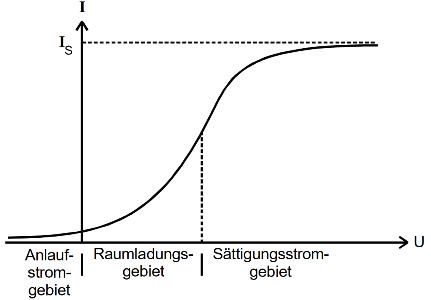
\includegraphics[width=\linewidth-70pt,height=\textheight-70pt,keepaspectratio]{content/images/Kennlinie.jpg}
\caption{Kennlinie eienr Hochvakuum-Diode\cite{V504}}
\label{fig:HVD}
\end{figure}